\documentclass[11pt,a4paper]{article}
\usepackage[utf8]{inputenc}
\usepackage[T1]{fontenc}
\usepackage{lmodern}
\usepackage[margin=1.8cm]{geometry}
\usepackage{graphicx}
\usepackage{hyperref}
\usepackage{enumitem}
\usepackage{titlesec}

\setlist{nosep,leftmargin=1.2em}
\titlespacing*{\section}{0pt}{0.4em}{0.2em}
\titleformat{\section}{\normalfont\bfseries\large}{\thesection}{0.5em}{}
\setlength{\parskip}{0.2em}
\setlength{\parindent}{0pt}

\title{\vspace{-1.5cm}Rapport individuel --- Itération 3}
\author{Alexis Briend (\texttt{abd7852}) --- Projet Long SHDL}
\date{23 mai 2026}

\begin{document}
\maketitle
\vspace{-2em}

\section*{Contexte}
Responsable de la \textbf{structure générale} et de l'\textbf{interprétation du SHDL} (\textsc{Scrum-23}). Sprint~3~: mener la conversion CST~$\to$~circuit de la combinatoire scalaire (sprint~2) jusqu'au \textbf{langage SHDL complet} --- vecteurs, appels de sous-modules, séquentiel (mémoire) --- puis assurer l'\textbf{intégration} de l'application (interface unifiée, build cross-OS).

\section*{Activités réalisées}
\begin{itemize}
  \item \textbf{Conversion vectorielle} (\texttt{Bus}, \texttt{Subset}, \texttt{Names})~: \texttt{ExpressionBuilder} vectorisé, LHS et paramètres vecteurs, peuplement de \texttt{Module.Entrees/Sorties} depuis la signature.
  \item \textbf{Appels de sous-modules multi-fichiers} (figure)~: \texttt{ModuleCallBuilder} (\texttt{ModuleCall}~$\to$~\texttt{AppelModule}), \texttt{ModuleResolver} + API \texttt{Conversion.convert(main, library)}, déduplication des LHS au bit physique. \textbf{Modules internes \texttt{\$}}~: \emph{dispatch} vers \texttt{BuiltinModules} (dont \texttt{\$BasculeD}).
  \item \textbf{Conversion séquentielle} (\texttt{:=})~: \texttt{MemoryAssignmentBuilder} (désucrage maître--esclave), \texttt{FreshNames} (signaux internes), réécriture des auto-références (compteurs)~; spec passée en revue adversariale.
  \item \textbf{Structure de l'app}~: intégration de notre interface (thème CSS clair/sombre) dans la branche de rendu, migration \textbf{JavaFX~25.0.3}, build \textbf{cross-OS} (Gradle/Makefile + GitHub Actions), correctifs IHM, suivi des bugs.
\end{itemize}

\begin{center}
\vspace{-0.4em}
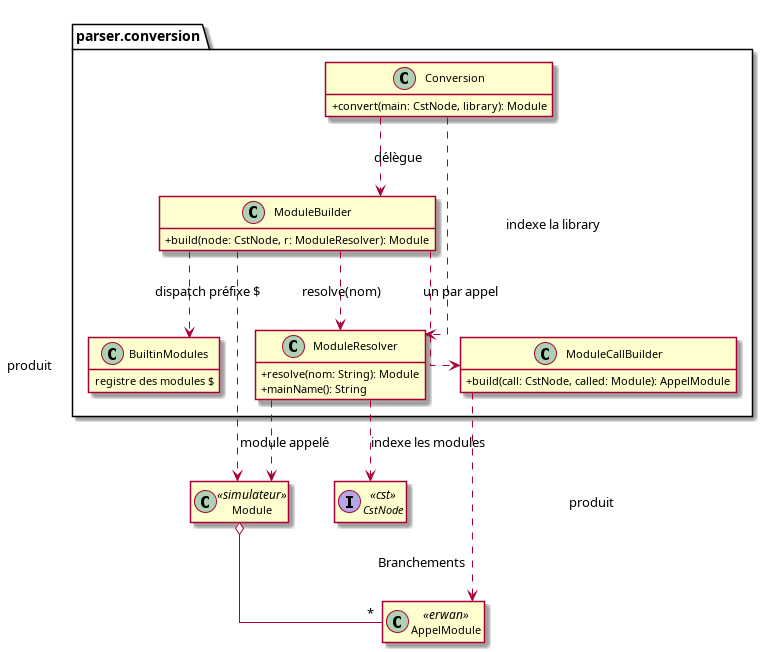
\includegraphics[width=0.46\textwidth]{../sous-modules-classes.png}\\
{\footnotesize Figure --- Conversion d'un appel de sous-module (\texttt{parser.conversion}).}
\vspace{-0.6em}
\end{center}

\section*{Résultats}
\begin{itemize}
  \item \textbf{Conversion menée à terme}~: 4~$\to$~\textbf{12 classes}, \textbf{127 tests JUnit} (14 classes de test)~; projet $\approx$\,389 tests (contre 193 au sprint~2). Pipeline SHDL complet~: scalaire, vecteurs, appels, mémoire.
  \item \textbf{Livrable cross-OS}~: \emph{build} vert sur les trois OS, archive packagée (jar + JavaFX + lanceur + exemples). Bug amont du simulateur isolé par un test reproducteur (\texttt{\$BasculeD}).
\end{itemize}

\section*{Difficultés et réussites}
Difficulté~: le désucrage maître--esclave de la séquentielle (\texttt{:=}) et les auto-références, sécurisés par revue adversariale et tests bout-en-bout. Réussite~: la \textbf{séparation stricte} parser~/~CST~/~conversion a tenu --- la conversion a grandi (vecteurs, appels, mémoire) sans toucher au parser.

\section*{Manuel utilisateur}
JDK~25. Pipeline~: \texttt{Conversion.convert(cst, library)} (\texttt{ConversionException} avec offset), puis \texttt{new FileSimulateur(m.Plan)}~; modules internes via préfixe \texttt{\$}. Build~: \texttt{make build} ou artefact CI par OS. Code sur \texttt{feature/parser-ll1-table-driven} et \texttt{apparence-build}.

\end{document}
